\section{Monday for MAT4002}\index{Monday_lecture}


\begin{theorem}
Let $\Gamma$ be a connected graph.
Then $\pi(\Gamma)$ is isomorphic to the free group generated by $\#\{E(\Gamma)\setminus E(T)\}$ elements,
for any maximal tree of $\Gamma$.
\end{theorem}
Now we give a proof for this theorem on one special case of $\Gamma$:
\begin{figure}[H]
\centering
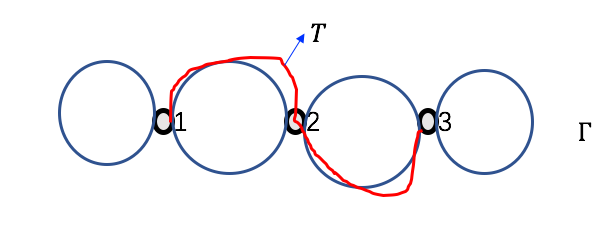
\includegraphics[width=0.5\textwidth]{week14/f_28}
\end{figure}
\begin{proof}
\begin{itemize}
\item
Fix an orientation for each $e\in E(\Gamma)\setminus E(T)$:
\begin{figure}[H]
\centering
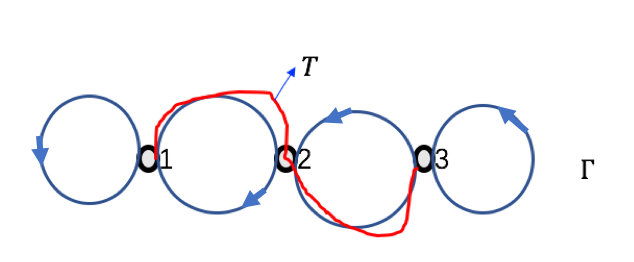
\includegraphics[width=0.5\textwidth]{week15/f_41}
\end{figure}
\item
Now let $K$ be a simplicial complex with $|K|\cong \Gamma$:
\begin{figure}[H]
\centering
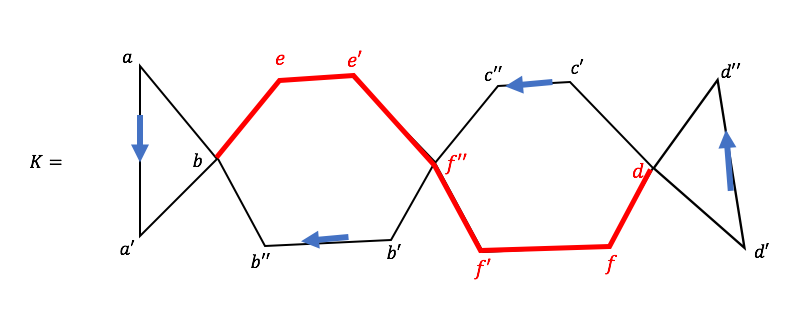
\includegraphics[width=0.5\textwidth]{week15/f_44}
\end{figure}
As a result, $E(K,b)\cong\pi_1(\Gamma)$
\item
Now we construct the group homomorphism
\[
\begin{array}{ll}
\phi:&\langle\alpha,\beta,\gamma,\delta\rangle\to E(K,b)\\
\text{with}&\phi(\alpha)=[ba'a''b]\\
&\phi(\beta)=[bee'f''b'b''b]\\
&\phi(\gamma)=[bee'f''f'fdc'c''f''e'eb]\\
&\phi(\delta)=[bee'f''f'fdd''d'dff'f''e'eb]
\end{array}
\]
\item
We can show the group homomorphism $\phi$ is bijective. In particular, the inverse of $\phi$ is given by:
\[
\begin{array}{ll}
\Psi:&E(K,b)\to\langle\alpha,\beta,\gamma,\delta\rangle\\
\end{array}
\]
where for any $[\ell]:=[bv_1\cdots v_n]\in E(K,b)$, the mapping $\Psi[\ell]$ is constructed by
\begin{enumerate}
\item[(a)]
Remove all other letters appearing in $\ell$ except $b,a',a'',b',b'',c',c'',d',d''$
\item[(b)]
Assign 
\[
\alpha,~~\alpha^{-1},~~\beta,~~\beta^{-1},~~\gamma,~~\gamma^{-1},~~\delta,~~\delta^{-1}
\]
for each appearance of 
\[
a'a'',~~a''a',~~b'b'',~~b''b',~~c'c'',~~c''c',~~d'd'',~~d''d',
\] 
respectively.
\end{enumerate}


\end{itemize}
\end{proof}





\subsection{The Selfert-Van Kampen Theorem}
\begin{theorem}
Let $K=K_1\cup K_2$ be the union of two \emph{path-connected open} sets, where $K_1\cap K_2$ is also path-connected.
Take $b\in K_1\cap K_2$, and suppose the group presentations for $\pi_1(K_1,b),\pi_1(K_2,b)$ are 
\[
\pi_1(K_1,b)\cong\langle X_1\mid R_1\rangle,\quad
\pi_1(K_2,b)\cong\langle X_2\mid R_2\rangle.
\]
Let the inclusions be
\[
i_1:K_1\cap K_2\xhookrightarrow{}K_1,\quad
i_2:K_1\cap K_2\xhookrightarrow{}K_2,
\]
then a presentation of $\pi_1(K,b)$ is given by:
\[
\pi_1(K,b) \cong\langle
X_1\cup X_2\mid 
R_1\cup R_2\cup 
\{(i_1)_*(g)=(i_2)_*(g): \forall g\in\pi_1(K_1\cap K_2,b)\}
\rangle.
\]
(Here $(i_1)_*:\pi_1(K_1\cap K_2,b)\xhookrightarrow{}\pi_1(K_1,b)$ and $(i_2)_*:\pi_1(K_1\cap K_2,b)\xhookrightarrow{}\pi_1(K_2,b)$.)
\end{theorem}


\begin{example}
\begin{enumerate}
\item
Let $K=S^1\wedge S^1$ given by
\begin{figure}[H]
\centering
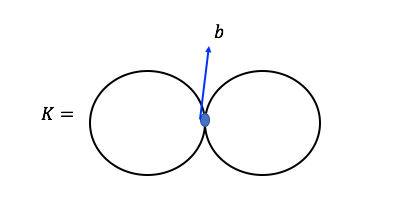
\includegraphics[width=0.4\textwidth]{week15/f_36}
\end{figure}
\begin{enumerate}
\item
Then construct $b$ as the intersection between two circles, and construct $K_1,K_2$ as shown below:
\begin{figure}[H]
\centering
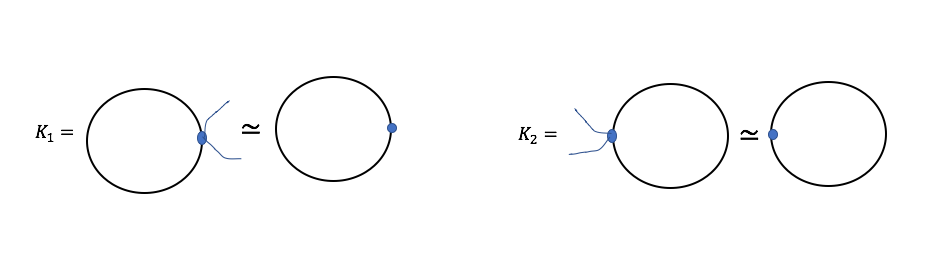
\includegraphics[width=\textwidth]{week15/f_37}
\end{figure}
We can see that $K_1\cap K_2$ is contractible:\begin{figure}[H]
\centering
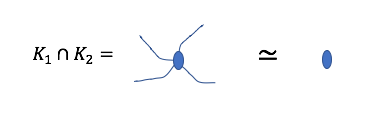
\includegraphics[width=0.4\textwidth]{week15/f_38}
\end{figure}
\item
As we have shown before, $\pi_1(S^1)\cong\mathbb{Z}$, which follows that
\[
\begin{array}{ll}
\pi_1(K_1,b)\cong\langle\alpha\rangle,
&
\pi_1(K_2,b)\cong\langle\beta\rangle
\end{array}
\]
Also, $\pi_1(K_1\cap K_2,b)\cong\pi_1(\{b\},b)\cong\{e\}$.
\item
It's easy to compute $(i_1)_*$ and $(i_2)_*$:
\[
\begin{array}{ll}
(i_1)_*:&\pi_1(K_1\cap K_2)\to\pi_1(K_1)\\
\text{with}&e\mapsto e
\end{array},\quad
\begin{array}{ll}
(i_2)_*:&\pi_1(K_1\cap K_2)\to\pi_1(K_2)\\
\text{with}&e\mapsto e
\end{array},
\]
\item
Therefore, by Seifert-Van Kampen Theorem,
\[
\pi_1(K,b)\cong\langle\alpha,\beta\mid e=e\rangle
\cong\langle\alpha,\beta\rangle
\]
\end{enumerate}
\item
By induction, 
\[
\pi_1(\wedge^n S^1,b)\cong\langle a_1,\dots,a_n\rangle
\]
For instance, the figure illustration for $\wedge^4 S^1$ and the basepoint $b$ is given below:
\begin{figure}[H]
\centering
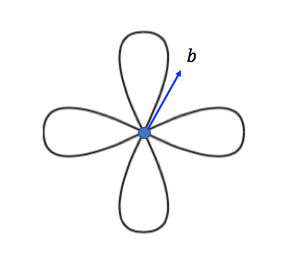
\includegraphics[width=0.3\textwidth]{week15/f_39}
\end{figure}

\item
\begin{enumerate}
\item
Construct $S^2=K_1\cup K_2$, which is shown below:
\begin{figure}[H]
\centering
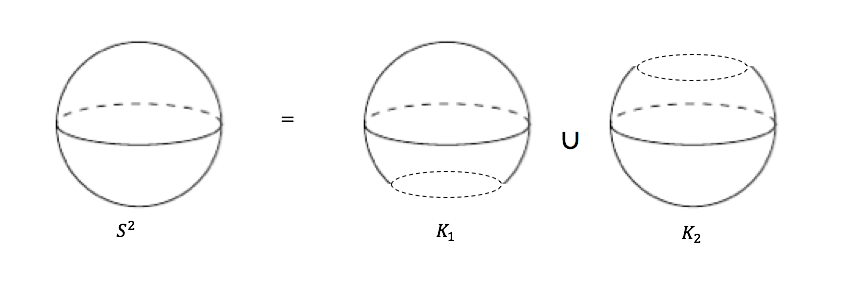
\includegraphics[width=0.8\textwidth]{week15/f_46}
\end{figure}
Therefore, we see that $K_1\cap K_2\simeq S^1$:
\begin{figure}[H]
\centering
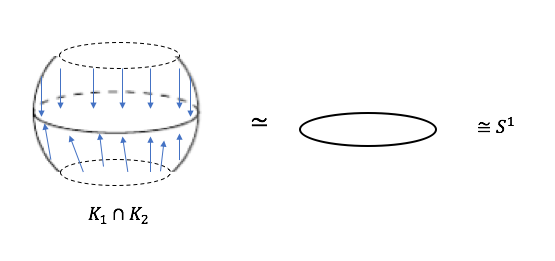
\includegraphics[width=0.5\textwidth]{week15/f_47}
\end{figure}
\item
It's clear that $K_1$ and $K_2$ are contractible, and therefore
\[
\begin{array}{ll}
\pi_1(K_1)\cong\langle\beta\mid\beta\rangle,
&
\pi_1(K_2)\cong\langle\gamma\mid\gamma\rangle
\end{array}
\]
and $\pi_1(K_1\cap K_2)\cong\pi_1(S^1)\cong\langle\alpha\rangle$.
\item
Then we compute $(i_1)_*$ and $(i_2)_*$.
In particular, the mapping $(i_1)_*$ is defined as
\[
\begin{array}{ll}
(i_1)_*:&\pi_1(K_1\cap K_2)\to \pi_1(K_1)\\
\text{with}&[\alpha]\mapsto[i_1(\alpha)]
\end{array}
\]
where $\alpha$ is any loop based at $b$. Since $K_1$ is contractible, we imply $\alpha$ in $K_1$ is homotopic to $c_b$, i.e., 
\[
(i_1)_*([\alpha]) = [i_1(\alpha)]=e,\forall \alpha\in \pi_1(K_1\cap K_2).
\]
Similarly, $(i_2)_*([\alpha])=e$.
\item
By Seifert-Van Kampen Theorem, we conclude that
\[
\pi_1(S^2) \cong \langle
\beta,\gamma\mid \beta,\gamma,e=e
\rangle
\cong
\{e\}
\]
\end{enumerate}

\item
Homework:
Use the same trick to check that $\pi_1(S^n) = \{e\}$ for all $n\ge 2$.
Hint: for $S^3$, construct
\[
K_1=\{(x_1,\dots,x_4)\in S^3\mid x_4>-1/2\}
\]
and
\[
K_1=\{(x_1,\dots,x_4)\in S^3\mid x_4<1/2\}
\]
\item
\begin{enumerate}
\item
Consider the quotient space $K\cong\mathbb{T}^2$, and we construct $K=K_1\cup K_2$ as follows:
\begin{figure}[H]
\centering
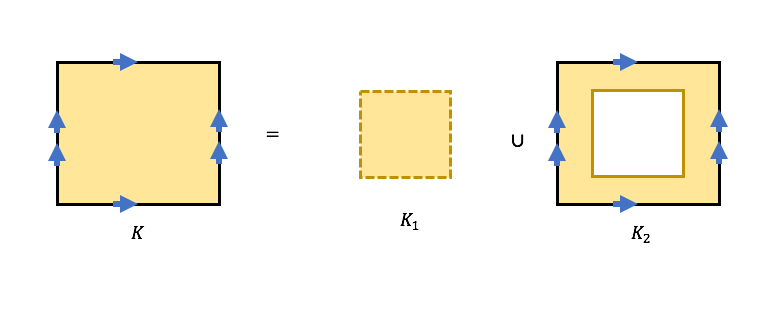
\includegraphics[width=0.5\textwidth]{week15/f_48}
\end{figure}

Therefore, we can see that $K_1$ is contractible, and $K_2$ is homotopy equivalent to $S^1\wedge S^1$:
\begin{figure}[H]
\centering
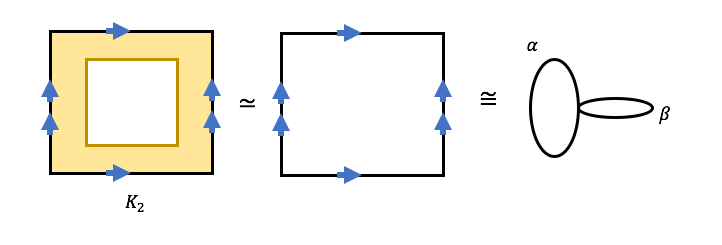
\includegraphics[width=0.6\textwidth]{week15/f_50}
\caption{Illustration for $K_2\simeq S^1\wedge S^1$}
\end{figure}
and $K_1\cap K_2$ is homotopic equivalent to the circle:
\begin{figure}[H]
\centering
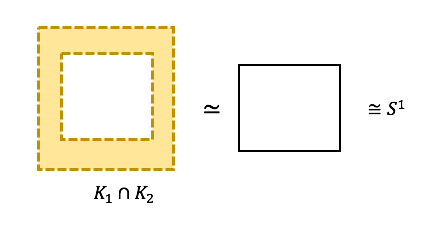
\includegraphics[width=0.6\textwidth]{week15/f_51}
\end{figure}

\item
It follows that
\[
\begin{array}{ll}
\pi_1(K_1)\cong\{e\},
&
\pi_1(K_2)\cong\langle \alpha,\beta\rangle,
\end{array}
\]
and $\pi_1(K_1\cap K_2)\cong \langle \gamma\rangle$.
\item
Then we compute $(i_1)_*$ and $(i_2)_*$.
In particular, $(i_1)_*$ is trivial:
\[
\begin{array}{ll}
(i_1)_*:&\pi_1(K_1\cap K_2)\to\pi_1(K_1)\\
\text{with}&[\alpha]\mapsto e
\end{array}
\]
Then compute $(i_2)_*$. In particular, for any loop $\gamma$, we draw the graph for $i_2(\gamma)$:
\begin{figure}[H]
\centering
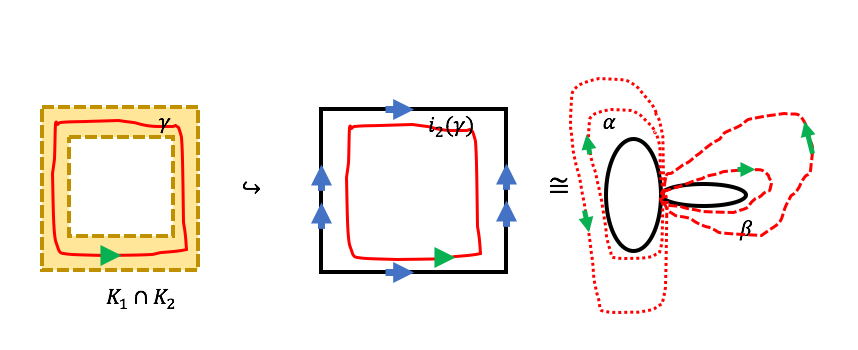
\includegraphics[width=0.6\textwidth]{week15/f_52}
\end{figure}
Therefore,
\[
(i_2)_*[\gamma]=[i_2(\gamma)]=[\alpha\beta\alpha^{-1}\beta^{-1}]
\]
\item
By Seifert-Van Kampen Theorem, we conclude that
\[
\pi_1(K) \cong \langle
\alpha,\beta\mid \beta,\alpha\beta\alpha^{-1}\beta^{-1}=e
\rangle
\cong
\langle
\alpha,\beta\mid ,\alpha\beta=\beta\alpha
\rangle\cong\mathbb{Z}\times\mathbb{Z}
\]
\end{enumerate}
\item
Exerise: The Klein bottle $K$ shown in graph below satisfies $\pi_1(K)=\langle a,b\mid aba^{-1}b\rangle$.
\begin{figure}[H]
\centering
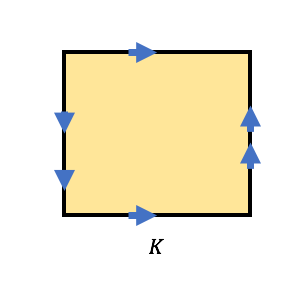
\includegraphics[width=0.4\textwidth]{week15/f_53}
\end{figure}
\item
Consider the quotient space $K=\mathbb{R}P^2$.
We construct $K=K_2\cup K_2$, which is shown below:
\begin{figure}[H]
\centering
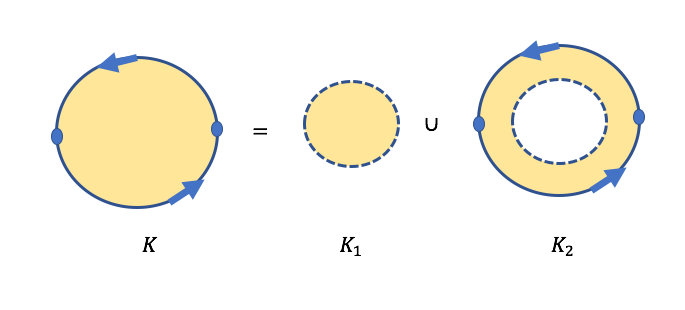
\includegraphics[width=0.4\textwidth]{week15/f_54}
\end{figure}
\begin{enumerate}
\item
It's clear that $K_1$ is contractible. In hw3, question 1, we can see that $K_2\simeq S^1$. Moreover, similar as in (5), $K_1\cap K_2\simeq S^1$.
\item
Therefore, $\pi_1(K_1)=\{e\}$ and $\pi_1(K_2)=\langle \alpha\rangle$, $\pi_1(K_1\cap K_2)=\langle \gamma\rangle$.
\item
It's easy to see that $(i_1)_*([\gamma])=e$ for any loop $\gamma$. 
For any loop $\gamma$, we draw the graph for $i_2(\gamma)$:
\begin{figure}[H]
\centering
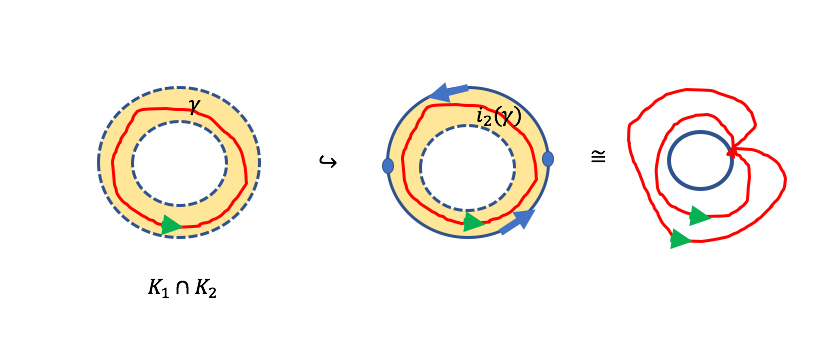
\includegraphics[width=0.4\textwidth]{week15/f_55}
\end{figure}
Therefore, $(i_2)_*([\gamma])=[i_2(\gamma)]=[\alpha^2]$.
\item
By Seifert-Van Kampen Theorem, we conclude that
\[
\pi_1(K) \cong \langle
\alpha\mid\alpha^2=e
\rangle
\cong
\mathbb{Z}/2\mathbb{Z}\cong\{0,1\}_{\bmod(2)}
\]
\end{enumerate}
\item
Let $K=\mathbb{R}^2\setminus\{\text{2 points $\alpha,\beta$}\}$. As have shown in hw3, $K\simeq S^1\wedge S^1$, which implies
\[
\pi_1(K)\cong\pi_1(S^1\wedge S^1)\cong\langle \alpha,\beta\rangle.
\]
We can compute the fundamental group for $K$ directly. Construct $K=K_1\cup K_2$ as follows:
\begin{figure}[H]
\centering
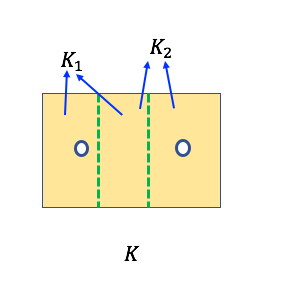
\includegraphics[width=0.3\textwidth]{week15/f_56}
\end{figure}
\begin{enumerate}
\item
It's clear that $K_1\cong\mathbb{R}^2\setminus\{\text{one point}\}\simeq S^1$ and similarly $K_2\simeq S^1$. Moreover, $K_1\cap K_2$ is contractible
\item
Therefore,
\[
\pi_1(K_1)\cong\langle\alpha\rangle,\quad
\pi_1(K_2)\cong\langle\beta\rangle,\quad
\pi_1(K_1\cap K_2)\cong\{e\}
\]
\item
Therefore, $(i_1)_*$ and $(i_2)_*$ is trivial since $\pi_1(K_1\cap K_2)\cong\{e\}$.
\item
By Seifert-Van Kampen Theorem, we conclude that
\[
\pi_1(K) \cong \langle
\alpha,\beta\mid e=e
\rangle
\cong
\langle
\alpha,\beta
\rangle
\]
\end{enumerate}


\end{enumerate}
\end{example}
























